\appendix

% Reinicia explícitamente el contador de capítulos
\setcounter{chapter}{0}

% Apéndice A - Tablas
\stepcounter{chapter}
\renewcommand{\thechapter}{Apéndice \Alph{chapter}}
\chapter*{Apéndice A: Tablas de referencia}
\addcontentsline{toc}{chapter}{Apéndice A: Tablas de referencia}
\markboth{Apéndice A: Tablas de referencia}{Apéndice A: Tablas de referencia}

\begin{table}[htbp]
\centering
\caption{Asociación entre nivel educativo de la madre y riesgo en dominios del desarrollo}
\label{tab:nivel_educativo_madre_desarrollo_anova}
\begin{threeparttable}
\begin{tblr}{
  width = 0.98\linewidth,
  colspec = {X[1.3,l]X[0.8,c]X[0.9,c]X[1.0,c]X[1.0,c]X[0.7,c]},
  row{1} = {font=\bfseries, bg=gray!10},
  row{even} = {bg=gray!3},
  cells = {valign=m, font=\footnotesize},
  hline{1,2,Z} = {1pt},
  hline{3-Y} = {0.5pt, gray},
}
\textbf{Dominio} & \textbf{F/W} & \textbf{\textit{p}-valor} & \textbf{Significativo} & \textbf{Método} & \textbf{N} \\
Comunicación          & 5.96   & $<$0.001  & Sí  & Welch's ANOVA & 1711 \\
Motricidad gruesa     & 6.29   & $<$0.001  & Sí  & ANOVA         & 1711 \\
Motricidad fina       & 8.68   & $<$0.001  & Sí  & ANOVA         & 1711 \\
Resolución de problemas & 9.51 & $<$0.001  & Sí  & ANOVA         & 1711 \\
Socio-individual      & 6.44   & $<$0.001  & Sí  & ANOVA         & 1711 \\
\end{tblr}
\begin{tablenotes}
\footnotesize
\item \textbf{Nota:}
El nivel educativo de la madre se asocia significativamente con todos los
dominios del desarrollo infantil. El grupo ``Universitario'' destaca por los
puntajes más altos y diferencias significativas con otros grupos; ``Ninguna escolaridad''
muestra los valores más bajos. El bajo nivel educativo materno es un factor
de riesgo importante para alteraciones en el neurodesarrollo infantil.
\end{tablenotes}
\end{threeparttable}
\end{table}

\begin{table}[htbp]
\centering
\caption{Asociación entre nivel educativo del padre y riesgo en dominios del desarrollo}
\label{tab:nivel_educativo_padre_desarrollo}
\begin{threeparttable}
\begin{tblr}{
  width = 0.98\linewidth,
  colspec = {X[1.4,l]X[0.8,c]X[1.0,c]X[1.0,c]X[1.0,c]X[0.7,c]},
  row{1} = {font=\bfseries, bg=gray!10},
  row{even} = {bg=gray!3},
  cells = {valign=m, font=\footnotesize},
  hline{1,2,Z} = {1pt},
  hline{3-Y} = {0.5pt, gray},
}
\textbf{Dominio} & \textbf{F/W} & \textbf{\textit{p}-valor} & \textbf{Significativo} & \textbf{Método} & \textbf{N} \\
Comunicación          & 6.82   & $<$0.001  & Sí  & ANOVA         & 1673 \\
Motricidad gruesa     & 1.88   & 0.114     & No  & Welch's ANOVA & 1673 \\
Motricidad fina       & 1.09   & 0.359     & No  & ANOVA         & 1673 \\
Resolución de problemas & 1.36 & 0.247     & No  & ANOVA         & 1673 \\
Socio-individual      & 2.57   & 0.036     & Sí  & ANOVA         & 1673 \\
\end{tblr}
\begin{tablenotes}
\footnotesize
\item \textbf{Nota:} El nivel educativo del padre se asocia significativamente con dos dominios del desarrollo infantil. Comunicación (F = 6.82, p $<$ 0.001, significativo) y Socio-individual (F = 2.57, p = 0.036, significativo). El grupo ``Ninguna escolaridad'' muestra los
valores más bajos y el grupo ``básico'' muestra la media de valores Z más alta.
\end{tablenotes}
\end{threeparttable}
\end{table}

\cleardoublepage
\stepcounter{chapter} 
\phantomsection
\addcontentsline{toc}{chapter}{Apéndice B: Permiso institucional}
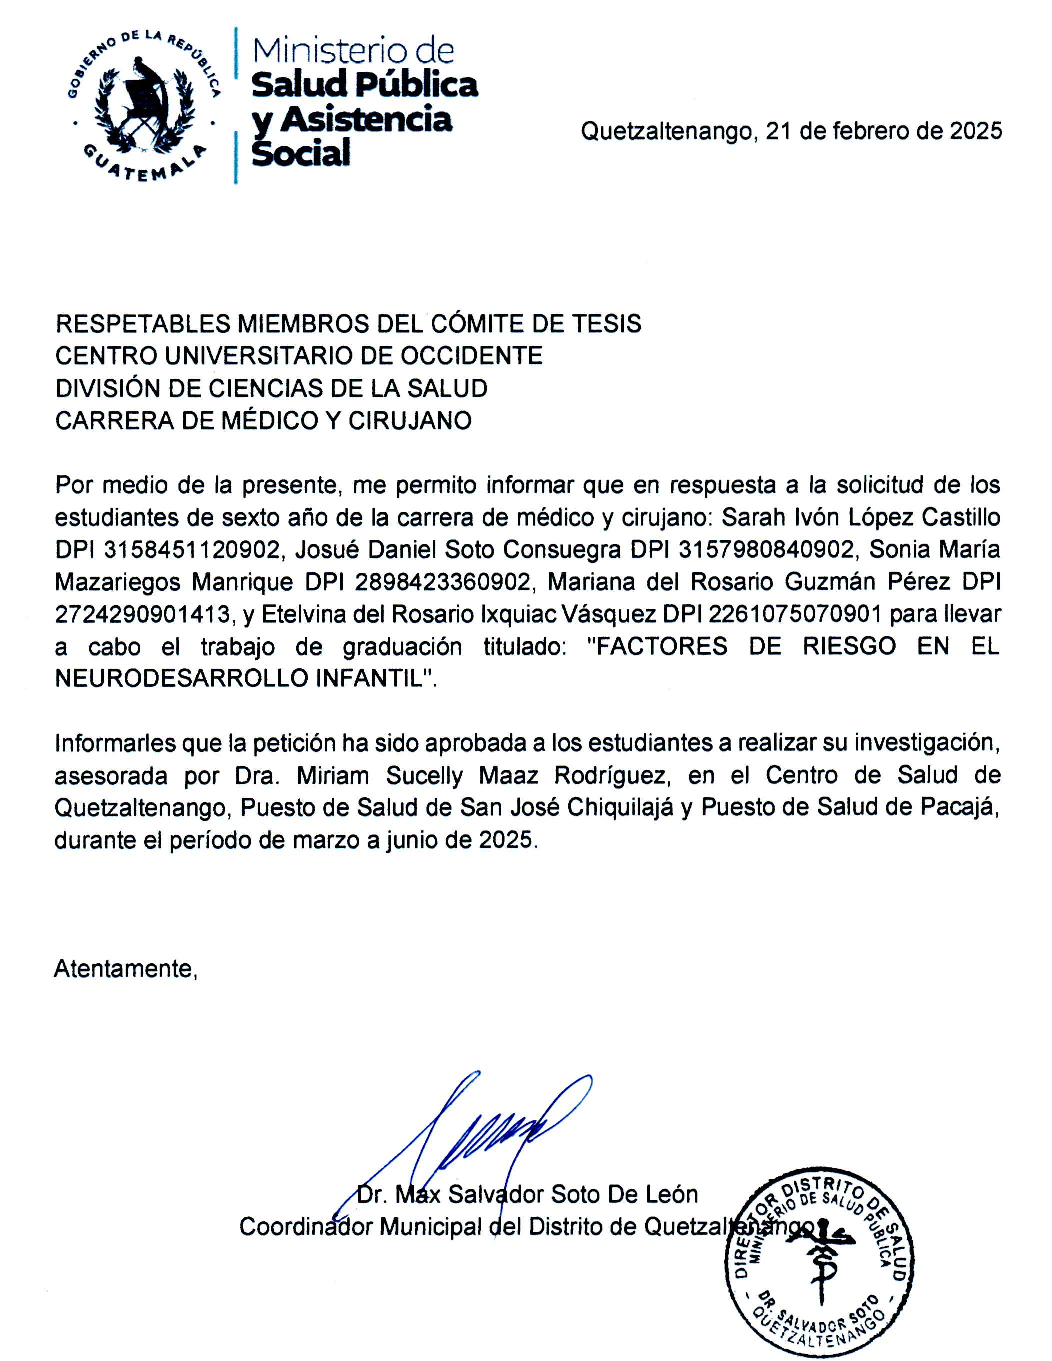
\includepdf[scale=0.78,pages=-,
  pagecommand={\thispagestyle{plain}\vspace*{0pt}\begin{center}\Large\bfseries Apéndice B: Permiso institucional\end{center}\vspace{1cm}}
]{varios/permiso.pdf}

\cleardoublepage
\stepcounter{chapter}
\phantomsection
\addcontentsline{toc}{chapter}{Apéndice C: Consentimiento informado}
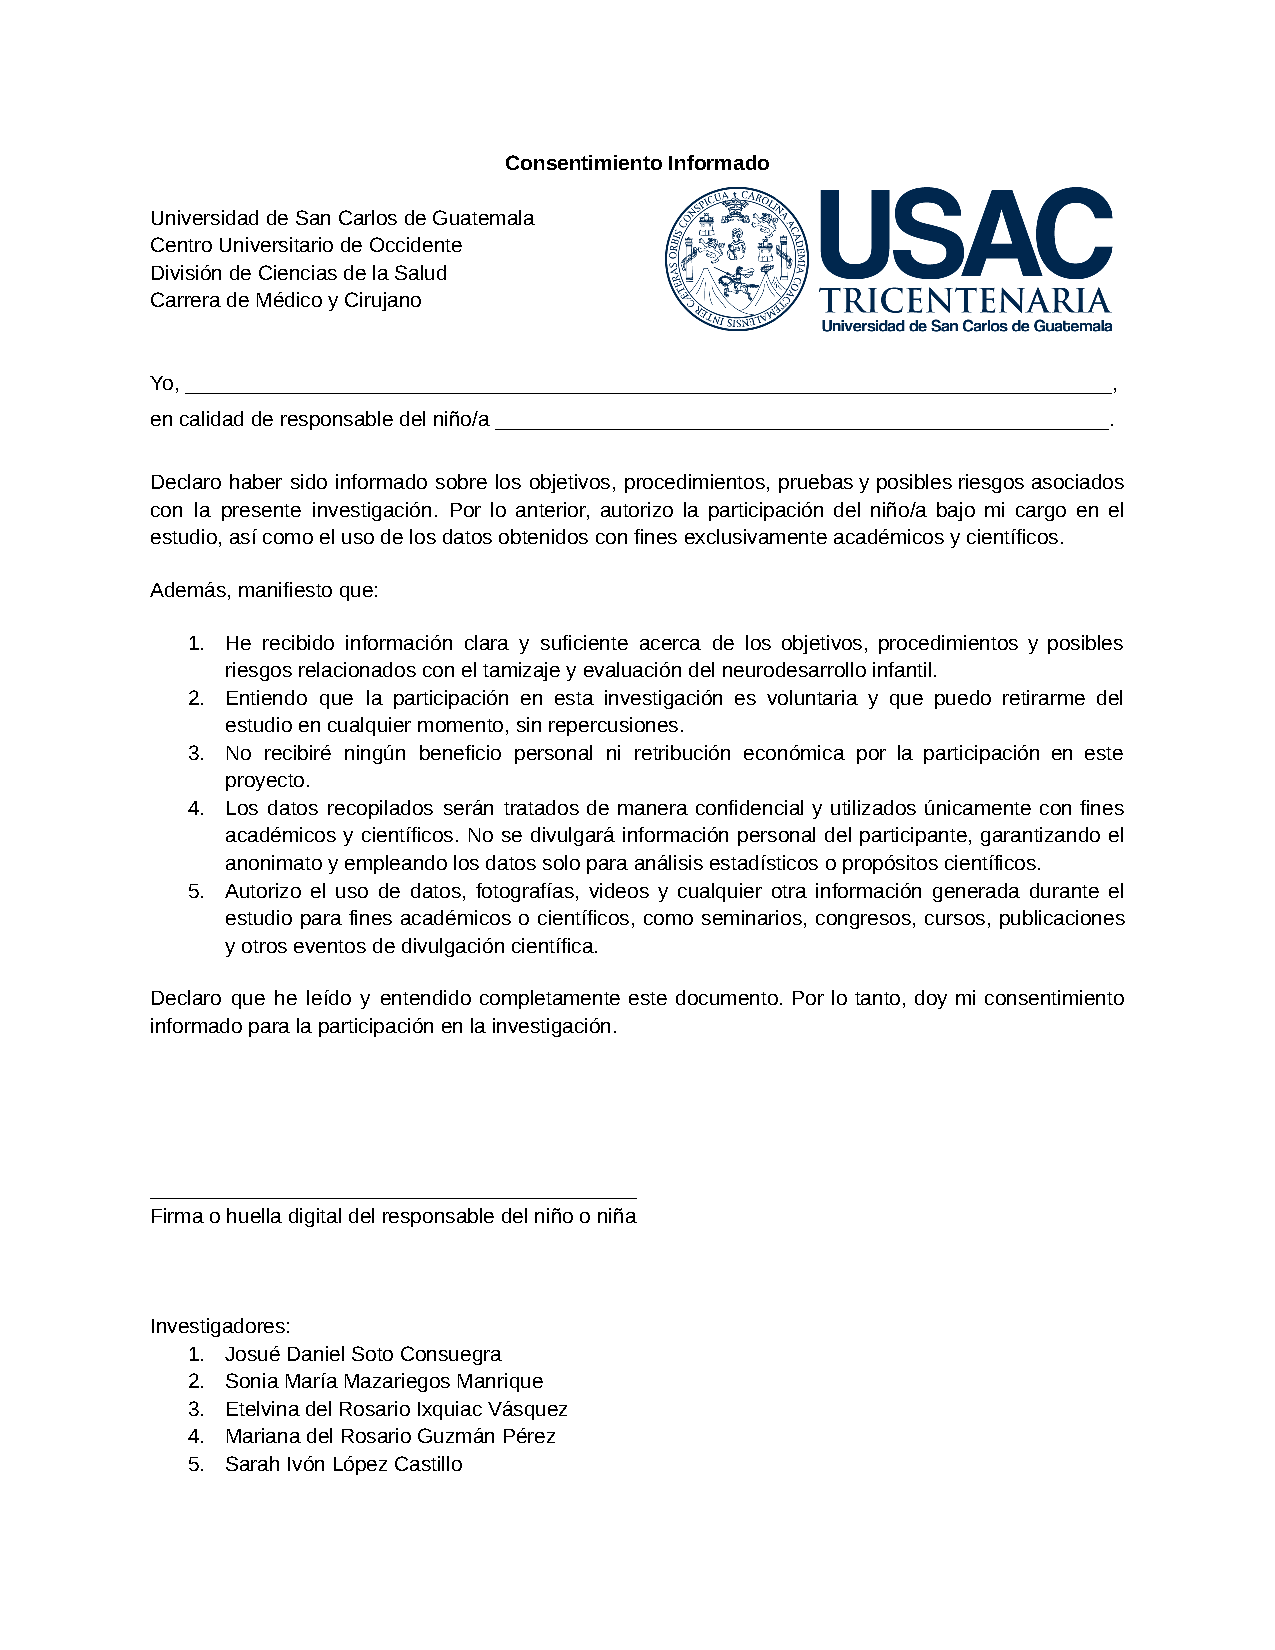
\includepdf[scale=0.9,pages=-,
  pagecommand={\thispagestyle{plain}\vspace*{0pt}\begin{center}\Large\bfseries Apéndice C: Consentimiento informado\end{center}\vspace{1cm}}
]{varios/consentimiento.pdf}

\cleardoublepage
\stepcounter{chapter}
\phantomsection
\addcontentsline{toc}{chapter}{Apéndice D: Boleta de recolección de datos}
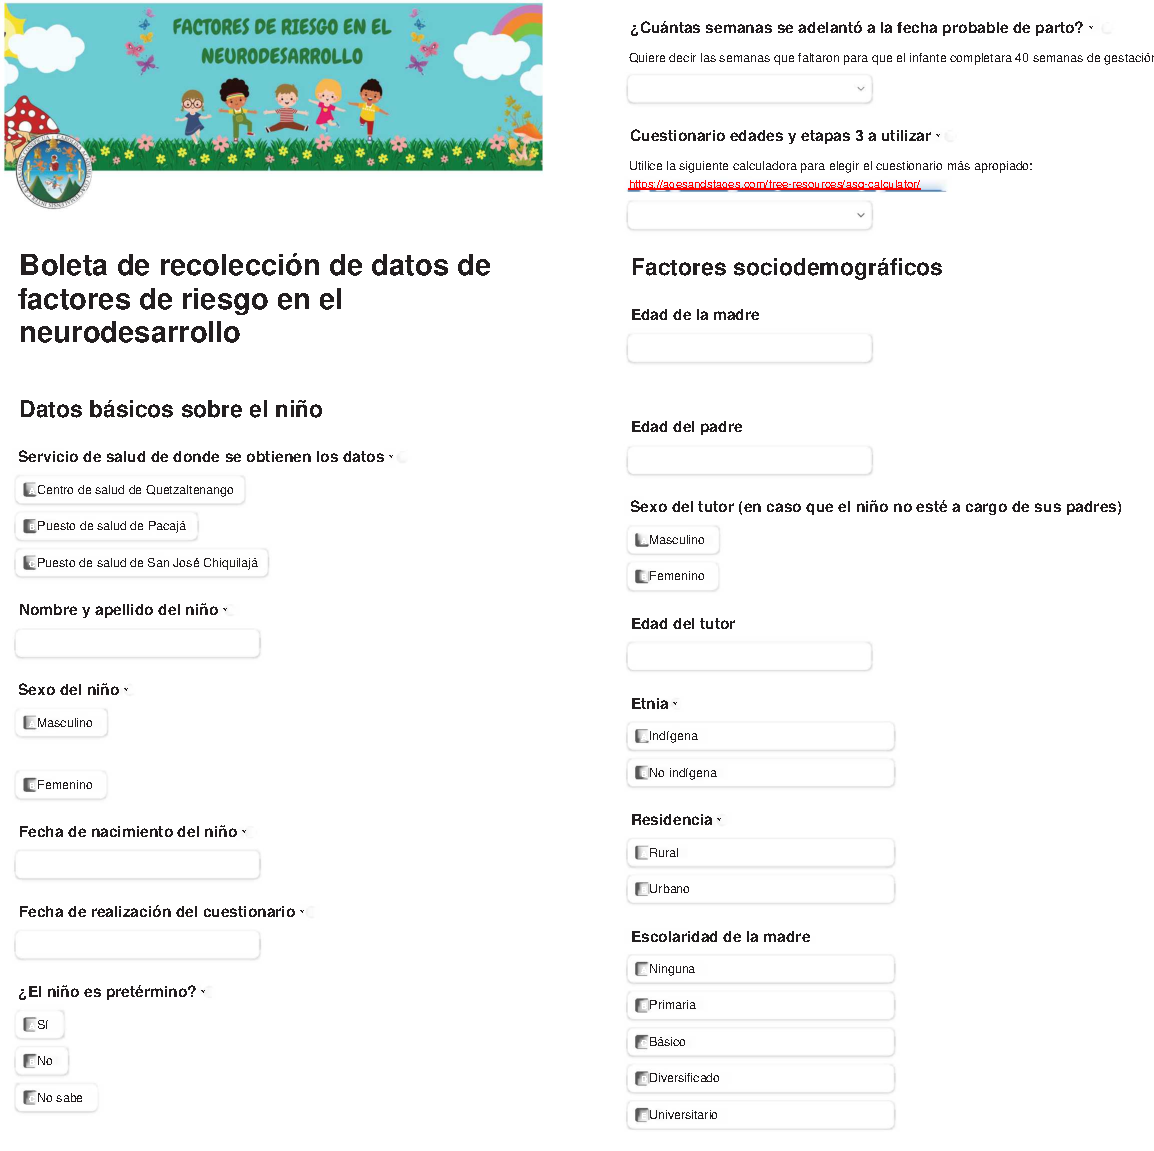
\includepdf[scale=0.85,pages=-,
  pagecommand={\thispagestyle{plain}\vspace*{0pt}\begin{center}\Large\bfseries Apéndice D: Boleta de recolección de datos\end{center}\vspace{1cm}}
]{varios/boleta.pdf}

\cleardoublepage
\stepcounter{chapter}
\phantomsection
\addcontentsline{toc}{chapter}{Apéndice E: Ejemplo de Cuestionario Edades y Etapas 3}
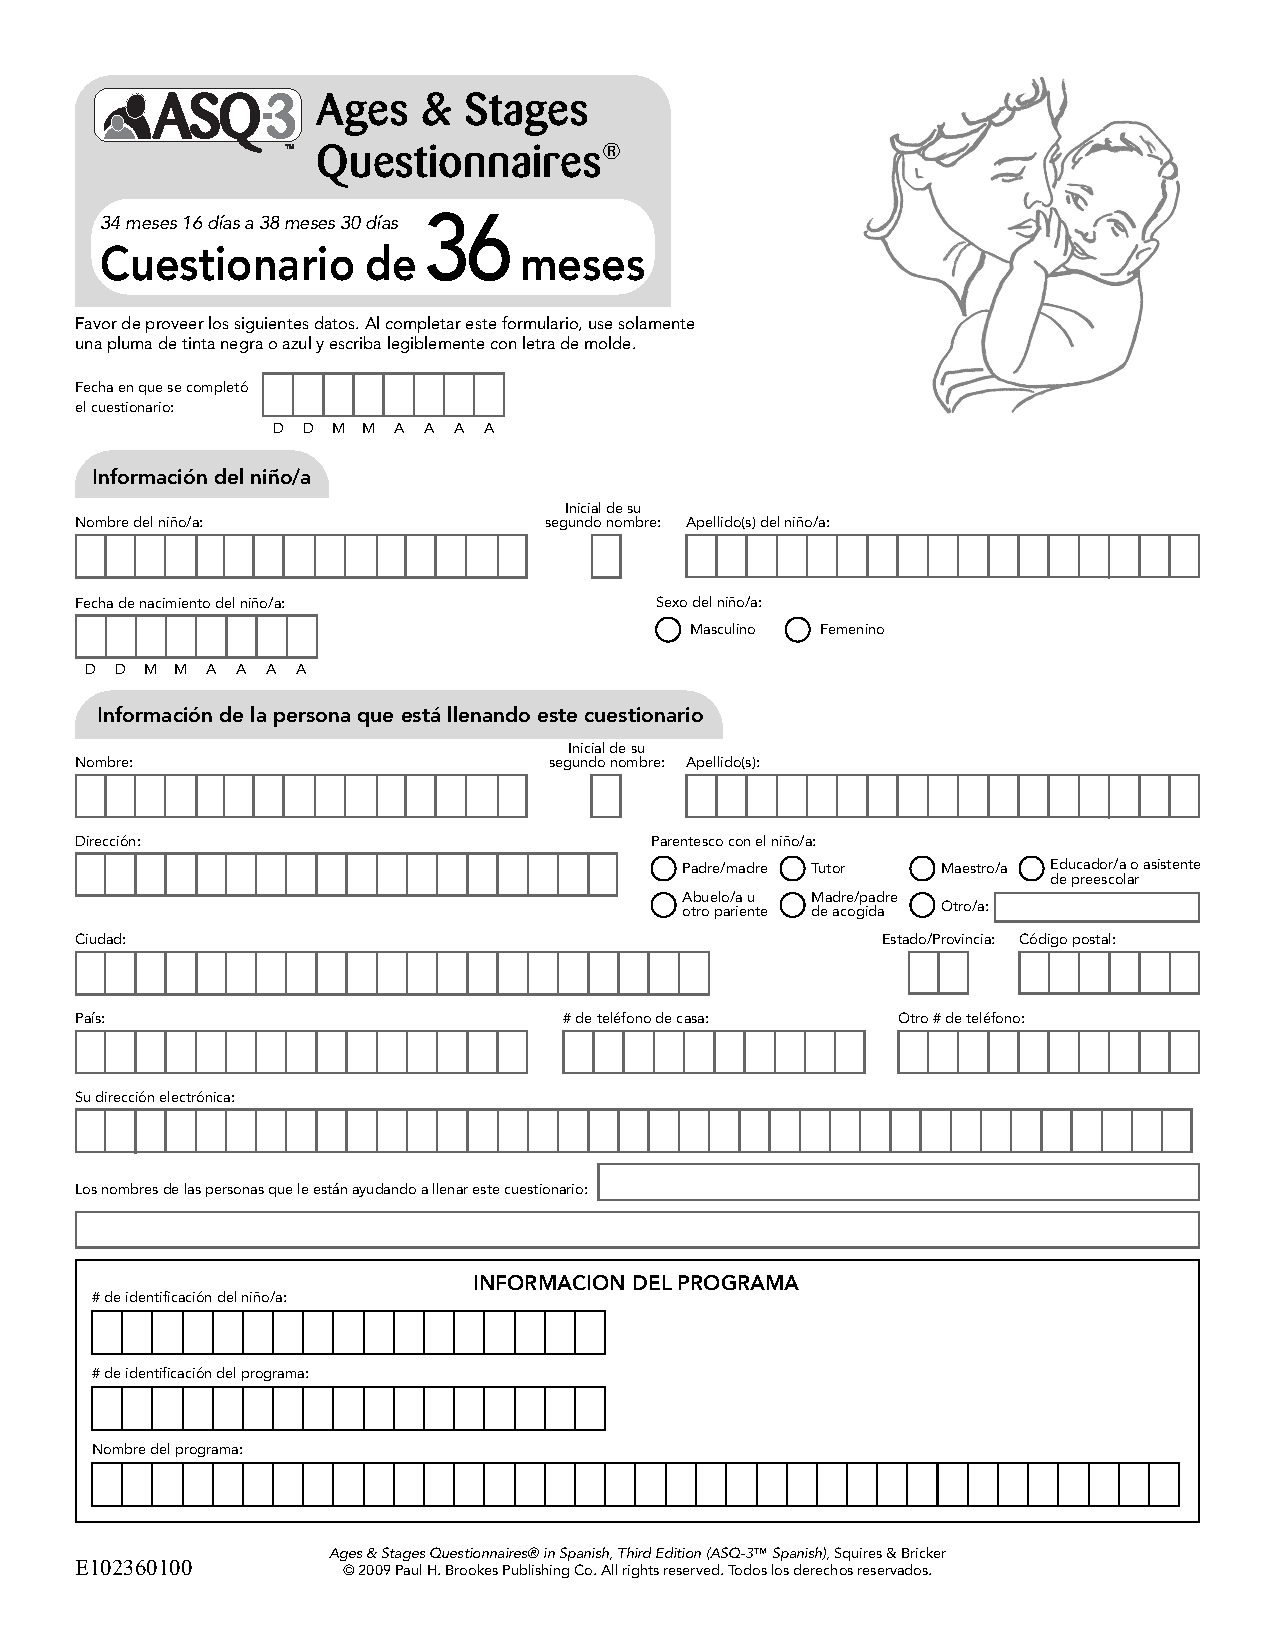
\includepdf[scale=0.80,pages=1-5,
  pagecommand={\thispagestyle{plain}\vspace*{0pt}\begin{center}\Large\bfseries Apéndice E: Ejemplo de Cuestionario Edades y Etapas 3\end{center}\vspace{1cm}}
]{varios/36meses.pdf}

\cleardoublepage
\stepcounter{chapter}

\phantomsection
\addcontentsline{toc}{chapter}{Apéndice F: Resultados de análisis de porcentaje de plagio}
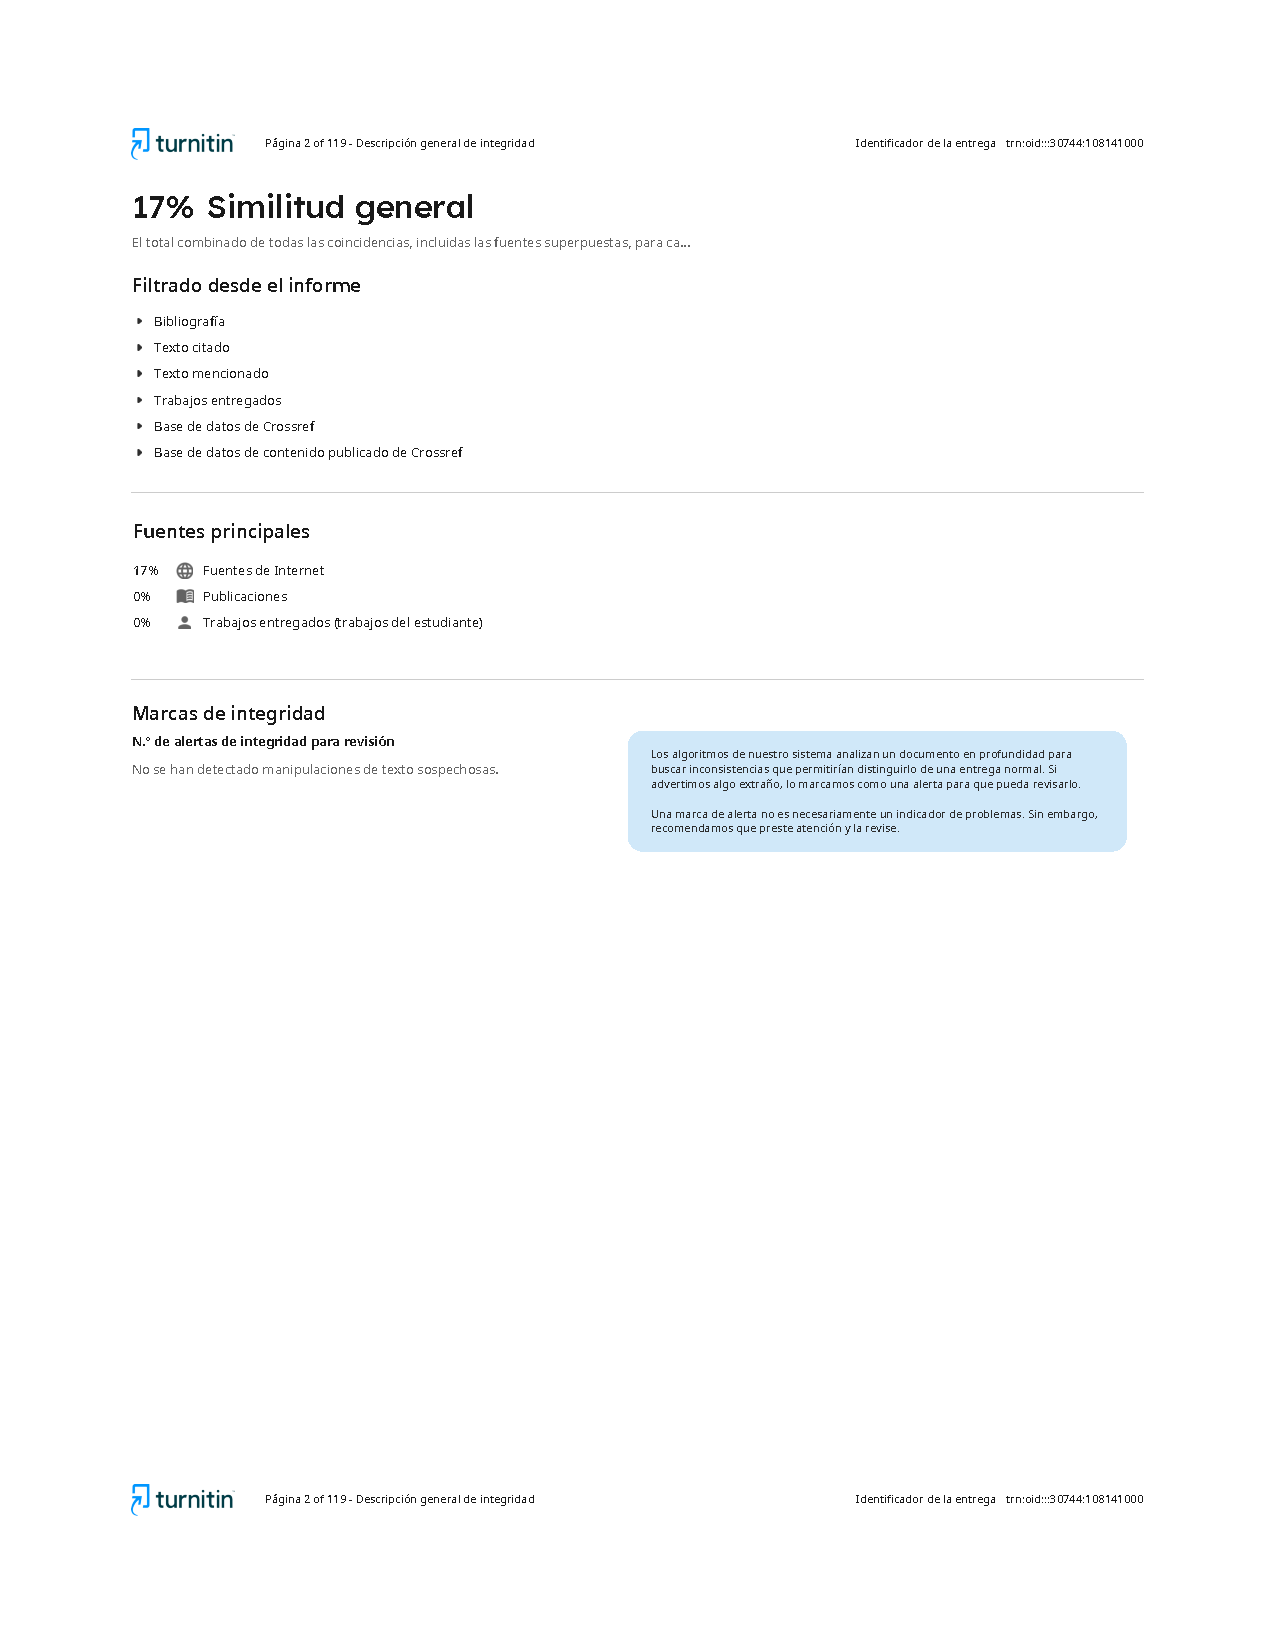
\includepdf[scale=0.80,
  pagecommand={\thispagestyle{plain}\vspace*{0pt}\begin{center}\Large\bfseries Apéndice F: Resultados de análisis de porcentaje de plagio\end{center}\vspace{1cm}}
]{varios/turnitin.pdf}
